\documentclass[../main.tex]{subfiles}

\begin{document}


\practica{3}{Entrada / Salida programada - UART TX}

    \subsection{Objetivos}
        \begin{itemize}
            \item Comprender más en profundidad el concepto de "periférico" dentro de un procesador.
            \item Aprender a programar un periférico.
            \item Interactuar con el periférico desde fuera de la placa.
        \end{itemize}

    \subsection{Fundamentos teóricos}

        \subsubsection{UART}

            La comunicación \textbf{UART} (\textit{Universal Asynchronous Receiver-Transmitter}) es un protocolo de comunicación serie asíncrono utilizado ampliamente en sistemas embebidos. Al ser asíncrono, no requiere de una señal de reloj compartida entre el emisor y el receptor; en su lugar, ambos dispositivos deben estar configurados previamente a la misma velocidad de transmisión (\textit{baud rate}).

            \textbf{Estructura de la Trama UART}: 
            
            En estado de reposo (\textit{Idle}), la línea de transmisión se mantiene en nivel lógico alto (\textbf{1}). Una trama estándar de datos está compuesta por los siguientes elementos:

            \begin{enumerate}
                \item \textbf{Bit de Inicio (\textit{Start Bit}):} Transición de nivel alto (\textbf{1}) a nivel bajo (\textbf{0}) durante un período de bit. Notifica al receptor que una nueva trama está comenzando.
                \item \textbf{Longitud de Palabra (\textit{Data Bits}):} Bloque de datos útil, transmitido habitualmente empezando por el bit menos significativo (\textit{LSB first}). Suele configurarse entre 5 y 9 bits, siendo 8 bits el valor más común.
                \item \textbf{Bit de Paridad (\textit{Parity Bit}, opcional):} Bit añadido al final de los datos para la detección elemental de errores:
                \begin{itemize}
                    \item \textbf{Paridad Par (\textit{Even}):} Se ajusta a 1 o 0 para que el número total de unos en la palabra de datos (incluyendo el bit de paridad) sea par.
                    \item \textbf{Paridad Impar (\textit{Odd}):} Se ajusta para que el número total de unos sea impar.
                \end{itemize}
                \item \textbf{Bits de Parada (\textit{Stop Bits}):} Uno o varios bits en nivel lógico alto (\textbf{1}) al final de la trama que garantizan un tiempo de resincronización mínimo para la línea antes de la siguiente transmisión.
            \end{enumerate}

            \textbf{Diagrama de Tiempos Típico}: 

            En la \Cref{fig:uart_frame} se muestra la representación gráfica de una trama serie de 8 bits de datos con paridad y 1 bit de stop:

            \begin{figure}[htbp]
            \centering
            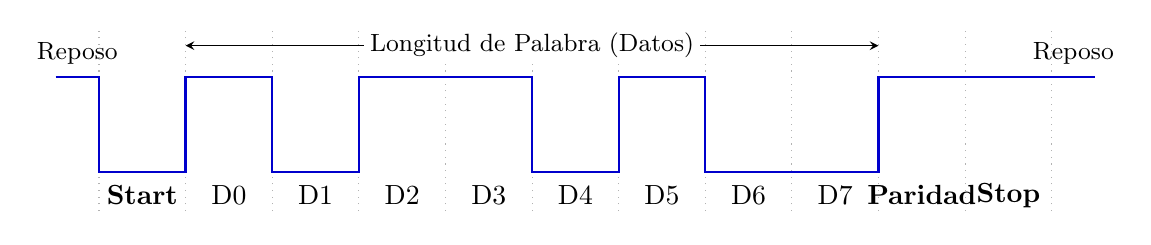
\begin{tikzpicture}[x=1.1cm, y=1cm, >=stealth]
                % Rejilla de tiempos/guías
                \draw[dotted, gray!60] (0,-0.5) -- (0,1.8);
                \draw[dotted, gray!60] (1,-0.5) -- (1,1.8);
                \draw[dotted, gray!60] (2,-0.5) -- (2,1.8);
                \draw[dotted, gray!60] (3,-0.5) -- (3,1.8);
                \draw[dotted, gray!60] (4,-0.5) -- (4,1.8);
                \draw[dotted, gray!60] (5,-0.5) -- (5,1.8);
                \draw[dotted, gray!60] (6,-0.5) -- (6,1.8);
                \draw[dotted, gray!60] (7,-0.5) -- (7,1.8);
                \draw[dotted, gray!60] (8,-0.5) -- (8,1.8);
                \draw[dotted, gray!60] (9,-0.5) -- (9,1.8);
                \draw[dotted, gray!60] (10,-0.5) -- (10,1.8);
                \draw[dotted, gray!60] (11,-0.5) -- (11,1.8);

                % Señal digital de ejemplo (Idle=1, Start=0, D0=1, D1=0, D2=1, D3=1, D4=0, D5=1, D6=0, D7=0, Parity=1, Stop=1, Idle=1)
                \draw[thick, blue!80!black] 
                    (-0.5, 1.2) -- (0, 1.2) 
                    -- (0, 0) -- (1, 0)       % Start Bit (0)
                    -- (1, 1.2) -- (2, 1.2)   % D0 (1)
                    -- (2, 0) -- (3, 0)       % D1 (0)
                    -- (3, 1.2) -- (5, 1.2)   % D2 (1), D3 (1)
                    -- (5, 0) -- (6, 0)       % D4 (0)
                    -- (6, 1.2) -- (7, 1.2)   % D5 (1)
                    -- (7, 0) -- (9, 0)       % D6 (0), D7 (0)
                    -- (9, 1.2) -- (10, 1.2)  % Paridad (1)
                    -- (10, 1.2) -- (11, 1.2) % Stop Bit (1)
                    -- (11.5, 1.2);           % Idle (1)

                % Etiquetas de bits
                \node at (-0.25, 1.5) {\small Reposo};
                \node at (0.5, -0.3) {\textbf{Start}};
                \node at (1.5, -0.3) {D0};
                \node at (2.5, -0.3) {D1};
                \node at (3.5, -0.3) {D2};
                \node at (4.5, -0.3) {D3};
                \node at (5.5, -0.3) {D4};
                \node at (6.5, -0.3) {D5};
                \node at (7.5, -0.3) {D6};
                \node at (8.5, -0.3) {D7};
                \node at (9.5, -0.3) {\textbf{Paridad}};
                \node at (10.5, -0.3) {\textbf{Stop}};
                \node at (11.25, 1.5) {\small Reposo};

                % Delimitadores superiores
                \draw[<->] (1, 1.6) -- (9, 1.6) node[midway, fill=white, inner sep=2pt] {\small Longitud de Palabra (Datos)};
            \end{tikzpicture}
            \caption{Cronograma de una trama de datos UART de 8 bits con paridad y 1 bit de parada.}
            \label{fig:uart_frame}
            \end{figure}
       
        \subsubsection{UART en el \MCU}

            En el procesador de la placa, se disponen de varios periféricos de UART diferentes, numerados como USARTx, siendo la x el número de UART. La UART dispone de varios registros de control, otros de configuración, y finalmente registros para la recepción/envío de datos. Todos ellos se describen en \REFMAN[27.8]. Las direcciones base de los periféricos USARTx se encuentran en \REFMAN[1.6.2]. Cómo hacer la transmisión en sí se describe en \REFMAN[27.5.2].

            ¿Ahora, qué USARTx utilizamos? en \BRDMAN[5.13] nos dice que la USART6 está conectada directamente a la salida desde ST-Link (El depurador que venimos utilizando hasta ahora para conectar con la placa). Por tanto, deberemos configurar USART6. Los pines donde se conecta (que habrá que activar) se pueden ver en \DSMAN[Table 10]. En concreto, vemos que son el pin PC6 para USART6\_TX y PC7 para USART6\_RX. (De momento solo usamos el TX para transmitir). Para que por ese pin salga la UART (Y no el valor genérico que ponemos en el puerto de salida del GPIO), deberemos configurar la función alternativa 8 como indica \DSMAN[Table 12], que conecta la USART6 al puerto C.

    \subsection{Desarrollo de la práctica}

        Para el desarrollo de esta práctica hay que extender el BSP introduciendo las funciones y definiciones necesarias de la UART, y posteriormente controlarla para emitir datos hacia el ordenador. La documentación necesaria puede verse en \REFMAN[27]. Los pasos a seguir son los siguientes:

        \begin{enumerate}
            \item Según \DSMAN[Table 10], el pin PC6 es quien saca al exterior la UART. Configúralo en modo de función alternativa en \REG{MODER}, tipo push-pull en \REG{OTYPER}, pull-up en \REG{PUPDR}, velocidad alta en \REG{OSPEEDR}, y configura la función alternativa en \REG{AFR} para que sea la 8 (como indica \DSMAN[Table 12]). No te olvides de activar el puerto C a través de \REG{AHB1ENR}.
            
                \begin{lstlisting}
                    RCC_AHB1ENR->bits.GPIOCEN = 1;
                    GPIO_MODE_SET(GPIOC, 6, GPIO_MODE_ALT);
                    //... completar
                \end{lstlisting}

            \item Ahora le toca el turno a la UART6 como nos indica \BRDMAN[5.13]. Actívala desde \REG{APB2ENR} lo primero.
            
                \begin{lstlisting}
                    //en bsp.h
                    #define RCC_APB2EN_BASE_ADDR 0x40023844
                    //Structure for Reset Control peripheral register APB1
                    typedef union {
                        volatile uint32_t reg;

                        // 2. Access individual bits or bit-groups for the register above
                        struct {
                            volatile uint32_t TIM1EN	   	: 1;  // Bit 0:
                            volatile uint32_t TIM8EN	   	: 1;  // Bit 1:
                            volatile uint32_t RES1		   	: 2;  // Bit 2-3:
                            //... completar
                        } bits;
                    } RCC_APB2R_TypeDef;
                    #define RCC_APB2ENR			((RCC_APB2R_TypeDef *) RCC_APB2EN_BASE_ADDR)

                    
                    //en main.c
                    RCC_APB2ENR->bits.USART6EN = 1; 		//enable UART clock
                \end{lstlisting}

            \item Configura la UART desde los registros \REG{CR1} y \REG{CR2} Activa el periférico, configura la longitud de palabra a 8 bits, 1 bit de stop y sin paridad, pone por último el oversampling a 16.
            \item Configura la velocidad de la UART desde \REG{BRR}. Tendrás que ponerle el valor del reloj del sistema (16MHz) entre la velocidad de la uart (115200).
            \item Por último, activa el modo de transmisión desde \REG{CR1}.
            
                \begin{lstlisting}
                    // UART STOP BITS
                    typedef enum {
                        UART_STOP_ONEBIT = 0x00,
                        UART_STOP_HALFBIT = 0x01,
                        UART_STOP_TWOBIT   = 0x02,
                        UART_STOP_ONEHALFBIT = 0x03
                    } UART_Stop_t;
                    #define UART_STOP_MASK 0b11
                    #define UART_STOP_SHIFT 12

                    static inline void UART_STOPBIT_SET(volatile USART_TypeDef *USARTx, UART_Stop_t stopbits) {
                        //... completar configurar el registro CR2 con los bits de stop
                    }

                    // UART ENABLE
                    typedef enum {
                        UART_DISABLE = 0x00,
                        UART_ENABLE = 0x01
                    } UART_Enable_t;
                    #define UART_ENABLE_MASK 0b1
                    #define UART_ENABLE_SHIFT 0

                    static inline void UART_ENABLE_SET(volatile USART_TypeDef *USARTx, UART_Enable_t enable) {
                        //... completar configurar el registro CR1 con el bit de enable
                    }

                    // UART WORD LENGTH
                    typedef enum {
                        UART_WORD_8B = 0x00,
                        UART_WORD_9B = 0x01,
                        UART_WORD_7B = 0x02
                    } UART_WordLength_t;
                    #define UART_WORD_MASK  0b1
                    #define UART_WORD_SHIFT 12

                    static inline void UART_WORDLENGTH_SET(volatile USART_TypeDef *USARTx, UART_WordLength_t length) {
                        //... completar escribir longitud en registro CR1
                    }

                    //... completar todas estas otras funciones auxiliares
                    static inline void UART_PARITY_SET(volatile USART_TypeDef *USARTx, UART_Parity_t parity);
                    static inline void UART_OVERSAMPLING_SET(volatile USART_TypeDef *USARTx, UART_Oversampling_t over);
                    static inline void UART_TX_MODE_SET(volatile USART_TypeDef *USARTx, UART_TX_Mode_t mode);
                \end{lstlisting}
            \item Cuando quieras transmitir un byte, espera primero a que quede libre el transmisor (aparece un 1 en el bit TC del registro \REG{ISR}. A continuación escribe el dato en el registro \REG{TDR}, la UART lo tramsmitirá solo.
            
                \begin{lstlisting}
                    //... en bsp.h
                    static inline void UART_TransmitByte(volatile USART_TypeDef *USARTx, uint8_t data)
                    {
                        while (!(USARTx->ISR & (1U << 7U))); //Wait until we can push data (TXE bit enabled)
                        USARTx->TDR = data; //push data (this clears TXE bit)
                    }


                    //... en main.c
                    UART_TransmitByte(USART6, 'X');
                    UART_TransmitByte(USART6, 'Y');
                    //...
                \end{lstlisting}
        \end{enumerate}
     
        Para ver ahora los mensajes desde el ordenador, utilizaremos la utilidad \texttt{picocom} (o cualquier otra terminal de vuestro gusto). Desde la máquina virtual, abrir una terminal y ejecutar el comando:

        \begin{lstlisting}
            picocom /dev/ttyACM0 -b 115200 -d 8 -y n -p 1
        \end{lstlisting}

        \textbf{NOTA:} El nombre del puerto puede no ser necesariamente \texttt{ttyACM0}, aunque en linux al menos es el valor por defecto. En Windows, por ejemplo, suele llamarse \texttt{COMx}, siendo x un número arbitrario.
        
        \subsubsection{Envío de cadenas de texto por UART}

            Aunque mola mucho programar en \emph{bare-metal}, también es útil partir de librerías ya implementadas para facilitar la vida a los programadores. Podemos ampliar la funcionalidad de nuestra UART para imprimir mensajes de depuración (así en próximas prácticas podremos depurar vía mensajes, en ocasiones más cómodo e intuitivo que la depuración con \emph{breakpoints}). Incluye las siguientes funciones y prueba a depurar tu código con mensajes.

            En \texttt{bsp.h} tendrás que añadir una función para escribir cadenas completas:

            \begin{lstlisting}
                void UART_WriteString(USART_TypeDef *usart, const char *str) {
                    while (*str) {
                        UART_TransmitByte(usart, *str++);
                    }
                }
            \end{lstlisting}

            En \texttt{main.c} tendrás que añadir la función de depuración en sí con las librerías necesarias auxiliares:

            \begin{lstlisting}
                #include <stdint.h>
                #include <stdlib.h>
                #include <stdio.h>
                #include <string.h>
                #include <stdarg.h>

                void Debug_Printf(const char *fmt, ...)
                {
                    char buf[256];
                    va_list args;
                    va_start(args, fmt);
                    vsnprintf(buf, sizeof(buf), fmt, args);
                    va_end(args);

                    UART_WriteString(USART6, buf);
                }
            \end{lstlisting}

            Y listo! Puedes llamar a la función \texttt{Debug\_Printf} con el texto con formato que quieras, para imprimir los valores de variables, por ejemplo, o simplemente colocar mensajes de depuración por la UART.

    \subsection{Para hacer más}

        Investiga las interrupciones de la UART para evitar tener que hacer esperas activas que consuman recursos de CPU. 




\end{document}